\chapter{Requisitos do Sistema}
% ---

Para que o sistema possa atender as demandas da Duas Rodas serão necessários alguns requisitos não só para um bom funcionamento do sistema, como também para tornar o projeto utilizável pela empresa, uma vez que os requisitos essenciais não sejam atendidos o projeto pode se tornar inviável para a implementação no setor da mecânica.
% ---


\section{Requisitos Funcionais}
% --- 
%O Smart Solution realizará o gerenciamento das ordens de serviço, distribuição delas via mobile para os mecânico, gerir a quantidade de peças no estoque, permitir que o mesmo solicite novas peças se necessário, consultar ordens de serviços de acordo com seu status (abertas, em andamento e finalizadas), armazenar assinaturas digitais através do número do crachá do funcionário, também possuirá funcionalidades extras como registro manual de funcionários e chamados de manutenção.
Os requisitos funcionais tratam de aspectos comportamentais do software.\cite{alvarenga2007abordagem}


\begin{figure}[H]
	\caption{\label{parte1funcional}Requisitos Funcionais Parte 1 Da \textit{Smart Solution}}
	\centering
	\mbox{%
		{
			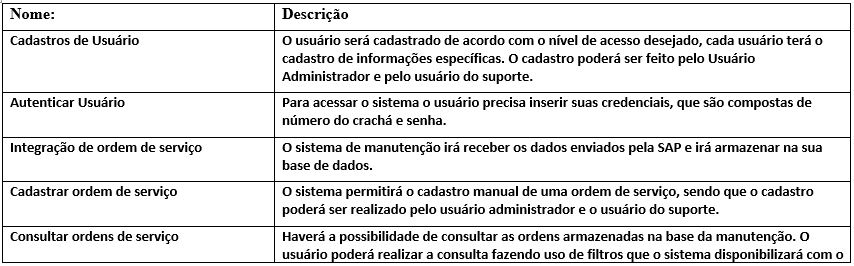
\includegraphics[scale=0.76]{Figuras/parte1funcional}}\qquad
		
	}
	
	
\end{figure}
\begin{figure}[H]
	\caption{\label{parte2funcional}Requisitos Funcionais Parte 2 Da \textit{Smart Solution}}
	\centering
	\mbox{%
		{
			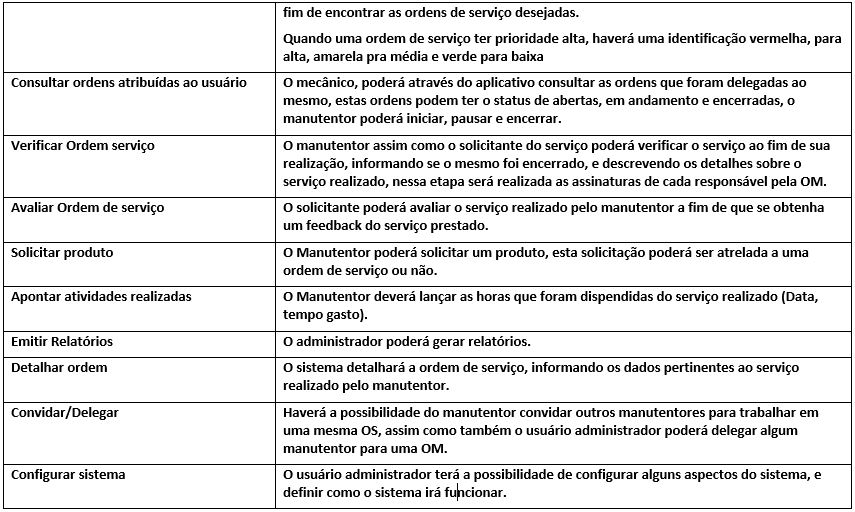
\includegraphics[scale=0.76]{Figuras/parte2funcional}}\qquad
		
	}
	
	
\end{figure}
\begin{figure}[H]
	\caption{\label{parte3funcional}Requisitos Funcionais Parte 3 Da \textit{Smart Solution}}
	\centering
	\mbox{%
		{
			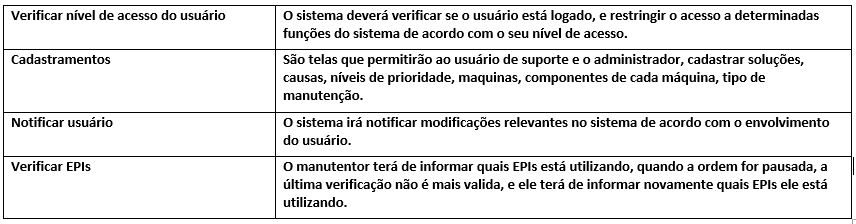
\includegraphics[scale=0.76]{Figuras/parte3funcional}}\qquad
		
	}
	
	
\end{figure}


%definiçao
%O \textit{Smart Solution} realizará o gerenciamento das ordens de serviço, distribuição delas via mobile para o mecânico, gerir a quantidade de peças no estoque, permitir que o mesmo solicite novas peças se necessário, consultar ordens de serviços de acordo com seu status (abertos, em andamento e finalizadas), armazenar assinaturas digitais através do número do crachá do funcionário, também possuirá funcionalidades extras como registro manual de funcionários e chamados de manutenção.



% ---
%\section{Requisitos Não-Funcionais}
% ---
\newpage
\section{Requisitos não Funcionais}
% ---
Os requisitos não-funcionais são as condições de comportamento e as restrições que 
Já os requisitos não-funcionais dizem respeito às condições de comportamento e restrições que devem prevalecer no software como, por exemplo, "o tempo de geração e emissão do relatório mensal que demonstra o histórico das transações comerciais de uma propriedade rural não deve ultrapassar 5 minutos". Neste exemplo, citamos um requisito de performance (ou um atributo de qualidade) que o software deve atender.\cite{alvarenga2007abordagem}


\begin{figure}[H]
	\centering
	\mbox{%
		{\label{reqnaofuncional}%
			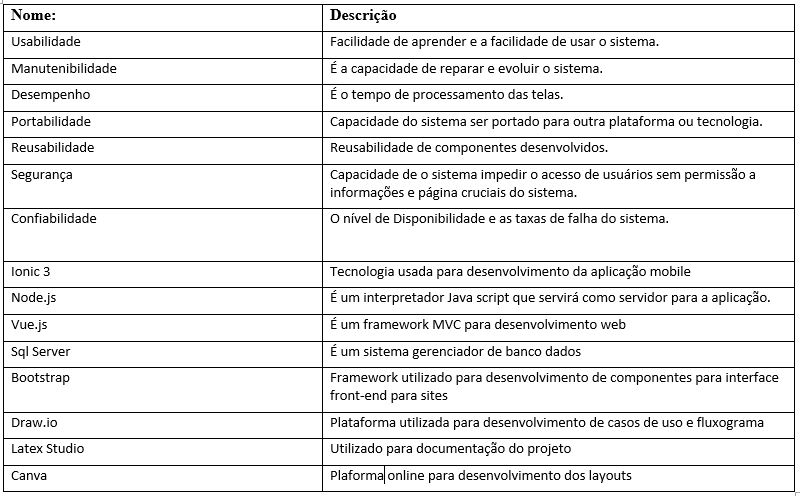
\includegraphics[scale=.80]{Figuras/reqnaofuncional}}\qquad
		

		}
	
	
\end{figure}
%(textyo a ser anexado)

% ---
\newpage
	


\section{Métricas}
% ---

Na concepção das ideias para desenvolver o \textit{Smart Solution}, foi utilizado primeiramente uma base fornecida pela empresa como as folhas de ordens de serviços, informações adicionais fornecidas no dia, após isso surgiu novas ideias como design, forma de colher as assinaturas, segurança, autenticação de usuário, ferramentas que melhor se encaixam com a proposta de software que seria desenvolvido. Agora as novas ideias são remover algumas telas e funcionalidades de teste que foram adicionadas na aplicação móvel, tais como: telas de cadastro de usuário e cadastro de ordem de serviço, e aplicá-las na versão web, pois caso algum recurso do SAP não estiver funcionando isso pode influenciar negativamente na abertura de chamados e integração com o \textit{Smart Solution}, dessa forma o sistema desenvolvido suprirá a parada inesperada do SAP ou qualquer outra fonte que afete a abertura de chamados. 
% ---
\newpage
\section{Cronograma}
% ---
Análise de requisitos, Planejamento, atribuição de tarefas,
desenvolvimento do layout do sistema, desenvolvimento da aplicação server,teste de implementação, finalização do projeto, testes para a implementação. Foram etapas para o desenvolvimento da documentação e implementação do projeto.


\begin{figure}[H]
	\caption{\label{Cronograma_marco_e_Abril}Cronograma para o desenvolvimento em março e Abril do projeto \textit{Smart Solution}}
	\begin{center}
		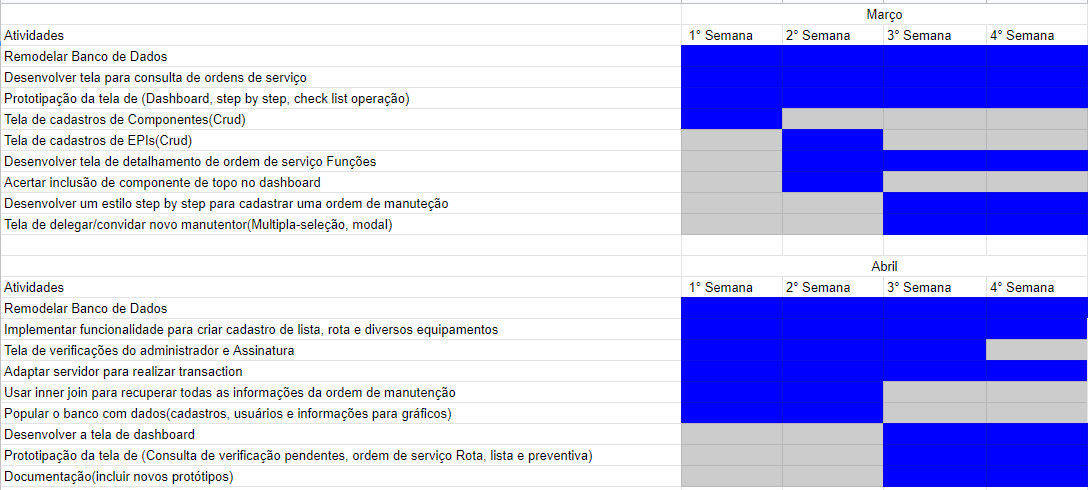
\includegraphics[scale=0.85,angle=90]{./Figuras/Cronograma_marco_e_Abril}
	\end{center}
	
\end{figure}
%----

\begin{figure}[H]
	\caption{\label{Cronograma_maio_e_Junho}Cronograma para o desenvolvimento em maio e junho do projeto \textit{Smart Solution}}
	\begin{center}
		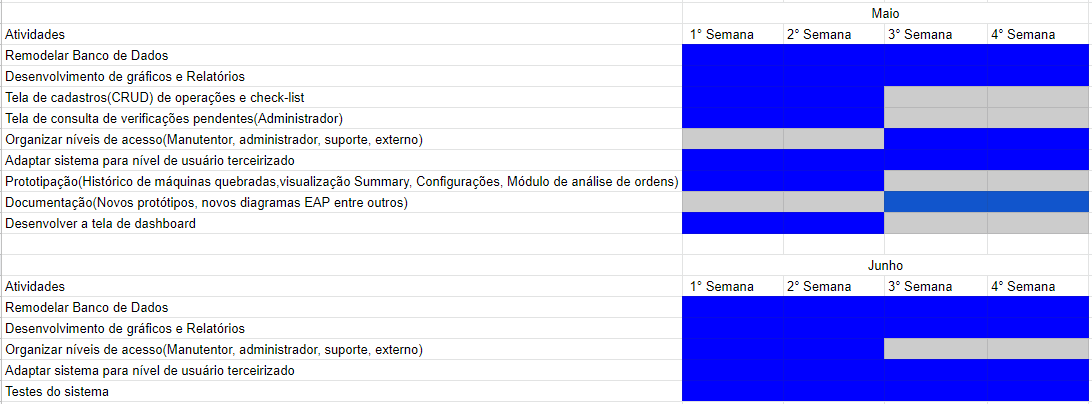
\includegraphics[scale=0.85,angle=90]{./Figuras/Cronograma_maio_e_Junho}
	\end{center}
	
\end{figure}
% ---
